% -*- TeX:de -*-
\NeedsTeXFormat{LaTeX2e}
\documentclass[12pt,a4paper]{article}
\usepackage[german]{babel} % german text
\usepackage[DIV12]{typearea} % size of printable area
\usepackage[T1]{fontenc} % font encoding
%\usepackage[latin1]{inputenc} % most likely on Windows
\usepackage[utf8]{inputenc} % probably on Linux
\usepackage{multicol}

% PLOTTING
\usepackage{pgfplots} 
\usepackage{pgfplotstable}
\usepackage{url}
\usepackage{graphicx} % to include images
\usepackage{tikz}
\usepackage{subfigure} % for creating subfigures
\usepackage{amsmath} % a bunch of symbols
\usepackage{amssymb} % even more symbols
\usepackage{booktabs} % pretty tables
\usepackage{makecell} % multi row table heading

% a floating environment for circuits
\usepackage{float}
\usepackage{caption}

%\newfloat{circuit}{tbph}{circuits}
%\floatname{circuit}{Schaltplan}

% a floating environment for diagrams
%\newfloat{diagram}{tbph}{diagrams}
%\floatname{diagram}{Diagramm}
\pgfplotsset{compat=1.8}
\selectlanguage{german} % use german

\begin{document}

%%%%%%% DECKBLATT %%%%%%%
\thispagestyle{empty}
			\begin{center}
			\Large{Fakultät für Physik}\\
			\end{center}
\begin{verbatim}


\end{verbatim}
							%Eintrag des Wintersemesters
			\begin{center}
			\textbf{\LARGE SS 14}
			\end{center}
\begin{verbatim}


\end{verbatim}
			\begin{center}
			\textbf{\LARGE{Physikalisches Praktikum\\ für das Bachelorstudium}}
			\end{center}
\begin{verbatim}




\end{verbatim}

			\begin{center}
			\textbf{\LARGE{PROTOKOLL}}
			\end{center}
			
\begin{verbatim}

\end{verbatim}

			\begin{flushleft}
			\textbf{\Large{Experiment (Nr., Titel): PS3 - Radioaktivität}\\
							%Experiment Nr. und Titel statt den Punkten eintragen
			\LARGE{PS3}}	
			\end{flushleft}

\begin{verbatim}

\end{verbatim}	
							%Eintragen des Abgabedatums, oder des Erstelldatums des Protokolls
			\begin{flushleft}
			\textbf{\Large{Datum:}} \Large{26.06.2014}
			\end{flushleft}
			
\begin{verbatim}
\end{verbatim}
							%Namen der Protokollschreiber
		\begin{flushleft}
			\textbf{\Large{Namen:}} \Large{Patrick Braun, Johannes Kurz}
			\end{flushleft}

\begin{verbatim}


\end{verbatim}
							%Kurstag und Gruppennummer, zb. Fr/5
			\begin{flushleft}
			\textbf{\Large{Kurstag/Gruppe:}} \Large{DO/4}
			\end{flushleft}

\begin{verbatim}

\end{verbatim}
							%Name des Betreuers, das Praktikum betreute.
			\begin{flushleft}
			\LARGE{\textbf{Betreuer:}}	\Large{Jonas Rodewald}	
			\end{flushleft}

%%%%%%% DECKBLATT ENDE %%%%%%%
\pagebreak
\setlength{\columnsep}{20pt}
\begin{multicols}{2}

%%%%%%%%%%%%%%%%%%%%%%%%%%%%%%%%%%%%%%%%%%%%%%%%

%\begin{figure}[H]
%	\centering
%	\includegraphics[scale=0.35]{./figure/beugung.png}
%	\caption{Beugungsmuster Einzelspalt (echtes Foto; schwarz durch weiß ersetzt)}
%	\label{fig:beugungsmuster}
%\end{figure}


%\begin{figure}[H]
%	\centering
%	\pgfplotstabletypeset[
%			columns={abstand, n},
%			col sep=&,
%			columns/abstand/.style={precision=2, zerofill, column name=\makecell{$Abstand$\\$(\pm 0.05)[mm]$} }, 
%			columns/n/.style={column name=\makecell{$n$\\$(Ordnung)$}, precision=0},
%			every head row/.style={before row=\hline,after row=\hline\hline},
%			every last row/.style={after row=\hline},
%			every first column/.style={column type/.add={|}{} },
%			every last column/.style={column type/.add={}{|} }
%			]{
%			abstand & n
%			12.9 & 1
%			24.45 & 2
%			37.40 & 3
%			49.35& 4
%			62.45 & 5
%			74.45 & 6
%			87.45 & 7
%			100.25 & 8
%			
%			}
%	\caption{Messwerte Einzelspalt}
%	\label{tab:werte_einzelspalt}
%\end{figure}


%%%%%%%%%%%%%%%%%%%%%%%%%%%%%%%%%%%%%%%%%%%%%%%%
%%%%%%%%%%%%%%%%%%%%%%%%%%%%%%%%%%%%%%%%%%%%%%%%


%\section{Schwingungen 2}
\noindent In PS3 werden die verschiedenen Arten von Radioaktivität untersucht. In den folgenden Versuchen werden einige Fragestellungen zu $\alpha-, \beta- und \gamma-Strahlung$ durch ausgewählte Experimente beantwortet.

%%%%%%%%%%%%%%%%%%%%%%%%%%%%%%%%%%%%%%%%%%%%%%%%%%%%%%%%%%%%%%%%%%%%%%%
\section{Grundlagen}
Es werden drei Arten von Strahlung unteschieden ([1] p.2):
\begin{itemize}
	\item $\alpha-Strahlung$: 2-fach positiv geladene Helliumkerne; sie haben aufgrund ihrer Masse die höchste Strahlungsenergie der 3 Arten.
	\item $\beta-Strahlung$: Elektronen oder Positronen; hauptsächlich entstehen sie beim Zerfall künstlicher radioaktiver Elemente;
	\item $\gamma-Strahlung$: hochenergetische Photonen; Sie entstehen bei $\alpha-$ und $\beta$-Zerfällen, wenn der angeregte Kern seine Energie wieder abgibt.
\end{itemize}

\noindent Radioaktive Strahlung hat eine ionisierende Wirkung und kann organisches Gewebe schwer beschädigen. Während $\alpha$-Strahlung nur eine sehr kurze Reichweite hat (wie im 4. Experiment gezeigt wird) und gut abgeschirmt werden kann, richten die $\alpha$-Teilchen im Körper aufgrund ihrer hohen Energie und der großen Wahrscheinlichkeit, andere Atome zu treffen, großen Schaden an. Jede Wechselwirkung regt außerdem wiederum Kerne an und führt so zu zusätzlicher $\gamma$-Strahlung und somit zu einer Kettenreaktion.\\
Auch $\beta$- und $\gamma$-Strahlung schädigt ZellenVor allem ein Großteil der $\gamma$-Strahlen geht zwar ungehindert durch den Körper, genauso lässt sich die Strahlung jedoch nur schwer abschirmen!\\

\noindent Daher ist in diesem Praktikums-Beispiel Sicherheit von großer Bedeutung.


\subsection{Radioaktiver Zerfall von Kupfer}
Der Zerfall einzelner Atome ist ein statistischer Prozess und für Atome gleicher Elemente gleich wahrscheinlich.  Pro Zeiteinheit zerfällt also eine gewisse Anzahl Kerne proportional zu ihrer Gesamtzahl. Daher kann ein einfaches Zerfallsgesetzt abhängig von der Gesamtanzahl der betrachteten Atome formuliert werden:
$$\frac{dN(t)}{dt} = -\lambda N(t)$$
oder als Lösung der Differentialgleichung:
$$N(t) = N_0 \cdot e^{-\lambda t}$$
Die Zerfallskonstante $\lambda$ ist abhängig vom Material. Außerdem ist die mittlere Lebensdauer $\tau = \frac{1}{\lambda}$ definiert. \\
Die Aktivität ist gegeben durch
$$A = \mid \frac{dN(t)}{dt} \mid = \lambda N(t) $$
Die Halbwertszeit, erhalten durch $N(t)/N_0 = 1/2$ ist:
$$T_{1/2} = \tau \cdot \ln 2 = \frac{\ln 2}{\lambda}$$


\subsection{Beta- und Gammaspektroskopie}

Nach einem $\beta$-Zerfall haben die Elektronen/ Positronen eine gewisse Energie, die teilweise an die anderen, am Zerfall beteiligten Teilchen abgegeben wird. Da dieser Prozess ein statistischer ist, ergibt sich ein kontinuierlich verteiltes Energiespektrum mit einer wahrscheinlichsten Energie $E_w$ und einer maximalen Energie $E_max$. Dieses $\beta$-Spektrum ist jedoch überlagert von $\gamma$-Strahlung, die beim $\beta$-Zerfall entsteht durch die angeregten Kerne.\\

\noindent Das $\gamma$-Spektrum überlagert das $\beta$-Spektrum und hat einen charakteristischen Verlauf aufgrund von Photoeffekt, Comptoneffekt und Paarbildung. Diese Effekte werden bei der Messung der Spektrums mittels Szintillationskristall benutzt:\\
\begin{itemize}
	\item Photoeffekt:\\
	Ein Photon trifft auf ein Elektron im Atom und überträgt seine Energie. Das Elektron wird aus dem Atom geschlagen (äußerer Photoeffekt) oder in einen höher-energetischen Zustand angeregt.
	\item Compton-Effekt:\\
	Ein relativ hochenergetisches Photon "streut" an einem freie Elektron; es gibt also seine Energie ab und es wird ein Photon mit anderer Wellenlänge (bedingt durch Impuls und Energieerhaltung abhängig vom Streuwinkel) erzeugt.
	\item Paarbildung:\\
	Hat ein Photon mehr Energie als die Summe der Ruheenergien eines Teilchen/Antiteilchen-Paares kann ein solches erzeugt werden. Die überschüssige Energie geht in die kinetische Energie der Teilchen ein.

\end{itemize}

\subsection{Abstandsgesetz für punktförmige Strahler}
Da jede Strahlungsquelle mit endlichen Abmessungen in ausreichender Entfernung als punktförmig angenommen werden kann, sollte das Abstandsgesetz für punktförmige Strahler auch für die Probe aus Aufgabe 2 gelten:
$$I(r) \propto \frac{1}{r^2}$$
Dieses Gesetz ergibt sich einfach aus der Geometrie des Problems, dass sich nämlich die Strahlung mit steigendem Abstand auf einer immer größer werdende Fläche verteilt.

\subsection{Reichweite von Alpha-Strahlen in Luft}

$\alpha$-Strahlung besteht aus doppelt positiv geladenen Heliumkernen. Sie geben ihre hohe Energie in einem Medium nicht auf einmal ab (wie Photonen) sondern verlieren sie laufend aufgrund von Stoßionisation mit den Teilchen.\\
In Luft verlieren sie ihre Energie in etwa $10^5$ bis $10^6$ Stößen. Da sie eine in etwa gleiche Anfangsenergie haben ergibt sich auch eine maximale Reichweite der $\alpha$-Teilchen.\\
In diesem Beispiel wird die Reichweite zum einen in der Nebelkammer gemessen, und zum anderen, näherungsweise berechnet mit der Formel:
$$R_m / mm = 3.1(E_{\alpha} / MeV)^{3/2}$$


%%%%%%%%%%%%%%%%%%%%%%%%%%%%%%%%%%%%%%%%%%%%%%%%%%%%%%%%%%%%%%%%%%%%%%%
\pagebreak
\section{Versuchsaufbau:}



\subsection{Radioaktiver Zerfall von Kupfer}

Im ersten Teil der Aufgabe soll die Radioaktivität im menschlichen Körper (verursacht durch Kalium-40) abgeschätzt werden. Dazu wird zuerst die Gesamtmenge an Kalium im Körper abgeschätzt und aus einer Nuklidkarte der Anteil an radioaktivem K-40 bestimmt. Ebenso aus der Karte kann die Halbwertszeit abgelesen werden und daraus die Zerfallskonstante berechnet werden und damit auch die Aktivität.\\

\noindent Der Hauptteil der Aufgabe ist es, die Halbwertszeit $T_{1/2}$, mittlere Lebensdauer $\tau$ und Zerfallskonstante $\lambda$ einer radioaktiven Kupferprobe zu bestimmen.\\
Die Zerfälle werden mit einem \emph{Geiger-Müller-Zählrohr} gemessen: Im GM-Zählrohr herrscht ein elektrisches Feld. Durch die ionisierende Strahlung entstehen positive und negative Ionen, die im E-Feld zur jeweiligen Elektrode hingezogen werden. Ist das Feld hinreichend stark, werden die Elektronen stark beschleunigt und ionisieren weitere Teilchen, die ebenfalls von den Elektroden eingefangen werden. So wird das Signal verstärkt (Gasverstärkung).\\
Die Ladungen an den Elektroden erzeugen eine Spannung, die gemessen werden kann. Mit einem Impulszähler wird jeder solcher Spannungsimpuls registriert und somit die Anzahl der Zerfälle gezählt.\\

\noindent Die Cu-Probe und das Zählrohr sind zur Abschirmung in einem Blei-Behälter. Da diese Abschirmung jedoch auch nicht 100\%-ig sein kann, wird, vor einbringen der Probe, die Strahlung im leeren Bleibehälter gemessen (Mittelwert aus 10 Messungen mit einer Messzeit von jeweils 100s). Diese Hintergrundstrahlung muss danach von der Cu-Messung abgezogen werden.\\
Die Messung der Zerfälle der Cu-Probe erfolgt computergestützt mit jeweils einem Messpunkt, alle 10 Minuten für etwa 4 Stunden.\\
Nach Bereinigung der Daten von der Hintergrundstrahlung werden die gesuchten Größen durch einen Fit ermittelt.

\subsection{Beta- und Gammaspektroskopie}

Zur Messung des Strahlungs-Spektrums einer unbekannten Proben wird ein Szintillationszähler verwendet:\\
Die zu messende Strahlung trifft auf einen Szintillationskristall und regt dort Elektronen an. Diese geben bei der Rückkehr in den Grundzustand wieder Strahlung ab.\\
Der Kristall ist ein NaI-Kristall, dotiert mit Thallium. Wird ein Thallium-Atom angeregt, reicht die abgegebene Strahlung nicht mehr aus, für weitere Anregungen und verlässt den Kristall.\\
Das Photon trifft auf eine Photokathode und löst dort eine gewisse, direkt zur Photonenenergie proportionale Anzahl an Elektronen aus. Diese werden wieder in einem anschließenden Verstärker vervielfacht und die so entstehende Spannung kann gemessen werden.\\
Aufgrund der Proportionalität der Energie zur Anzahl der Elektronen und damit zur Spannung, kann der Szintillationszähler, im Gegensatz zum GM-Zähler, ein Spektrum aufnehmen.\\

\noindent Anhand des charakteristischen $\gamma$-Spektrums kann die unbekannte Probe identifiziert werden.

\subsection{Abstandsgesetz für punktförmige Strahler}

Zum Nachweis des Strahlungsgesetzes wird die Probe aus Aufgabe 2 im Szintillationszähler belassen und mehrere Spektren bei verschiedenen Abständen vom Kristall genommen.\\
Um den Zusammenhang deutlich zu zeigen, werden die Abstände quadratisch ansteigend gewählt und die Strahlung gegen die reziproken Abstandsquadrate aufgetragen.\\
Um die Intensität quantitativ gut zu erfassen, werden beide charakteristischen Strahlungspeaks der Probe verwendet: pro Abstand werden beide Peaks mit einer Gausskurve gefittet (nach Bereinigung der Hintergrundstrahlung, die zuvor gemessen wurde) und diese integriert.\\
Auf diese Weise werden die statistischen Schwankungen der Zerfälle geglättet und "summiert". Dies ist ein Maß für die Intensität, die für den Nachweise des Abstandsgesetzes nur in relativen Werten benötigt wird.

\subsection{Reichweite von Alpha-Strahlen in Luft}

Eine radioaktive Probe (Ra 226) wird in eine Nebelkammer eingebracht. Darin sorgt eine hohe Saugspannung für eine Beschleunigung der $\alpha$-Teilchen in eine bestimmte Richtung (zur leichteren Beobachtbarkeit). Die $\alpha$-Teilchen ionisieren Teilchen des Nebels, die dann als Kondensationskeime wirken und somit als Nebelspur den Weg der Strahlung nachzeichnen.\\
Als Nebel wird Ethanol-Dampf verwendet, der entsteht, indem Ethanol, mit flüssigem Stickstoff stark heruntergekühlt, am Boden der Kammer, und sich weiter oben in der Kammer, Ethanol bei Raumtemperatur befindet.\\
Durch das Temperaturgefälle entsteht nahe des Bodens übersättigter Ethanol-Dampf.\\

\noindent Von den Nebelspuren wird anschließend ein Photo gemacht, und die maximale Reichweite der Teilchen (in Relation zum bekannten Durchmesser der Probe - 1cm) gemessen.\\
Verglichen wird das Ergebnis mit dem Ergebnis der Näherungsformel.


%%%%%%%%%%%%%%%%%%%%%%%%%%%%%%%%%%%%%%%%%%%%%%%%%%%%%%%%%%%%%%%%%%%%%%%
\pagebreak
\section{Resultate}
\subsection{Radioaktiver Zerfall von Kupfer}
\end{multicols}
\begin{figure}[H]
	\centering
	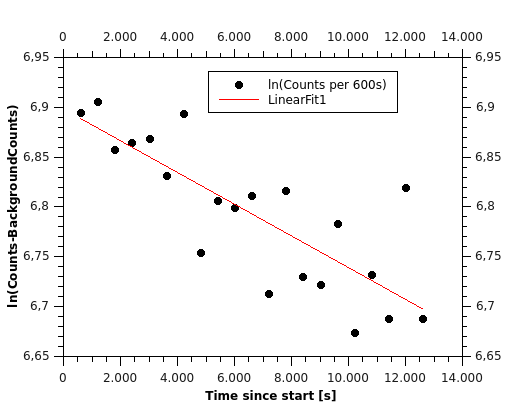
\includegraphics[scale=2.5]{./figures/kupfer_zerfall_ergebnis.png}
	\caption{Logarithmus der Aktivität gegen Zeit, Steigung entspricht $\lambda$}
	\label{fig:kupferzerfall_erg}
\end{figure}
\begin{multicols}{2}
% $\lambda$ = (-1.591120669338278 \pm 0.2686603661676406) E-05
\noindent Hintergrundstrahlung:\\
$(12.0 \pm 2.4) counts/ 100s$\\

 \noindent aus dem Fit:\\
$\lambda = (1.6 \pm 0.3)\times10^{-5}s^{-1}$\\
 $\tau = (17.46 \pm 2.43)h$\\
 %(ln(2)/0.00001591120669338278)/60/60
 $$T_{1/2} = (12.1 \pm 2.1)h$$
(Literaturwert: $T_{1/2} ({64}^{Cu}) = 12.701(2) h$)
 Quelle: [3]\\

\noindent \textbf{Körpereigene Radioaktivität:}\\
Kalium in 70kg Mensch: $\sim 140g$\\
K-40 Anteil in natürlichem K: $\sim 0.0117\%$\\
a) K-40 im Menschen (70kg): $\sim 0.01638$g\\
b) K-40 Atome im Körper: $\sim 2.468 \times 10^{20}$\\
c) $T_{1/2} = 1.248 \times 10^9$ Jahre\\
$\lambda = 1.761 \times 10^{-17}s^{-1}$\\

\noindent d) Einsetzen in die Aktivität (bei ungefährt konstantem Kaliumanteil im Körper, bedingt durch den Stoffwechsel):\\
$$A = \lambda \cdot N_0 = (4350 \pm 435) Bq$$



\subsection{Beta- und Gammaspektroskopie}

\subsection{Abstandsgesetz für punktförmige Strahler}
verwendete Energieintervalle:\\
Peak 1: 1117keV - 1256keV\\
Peak 2: 1260keV - 1409keV\\

\noindent Abstände der Probe vom Kristall:\\ 
$(5.59 \pm 0.01)cm$\\
$(6.09 \pm 0.01)cm$\\ 
$(7.05 \pm 0.01)cm$\\
$(8.99 \pm 0.01)cm$\\
$(13.00 \pm 0.01)cm$\\
\begin{figure}[H]
	\centering
	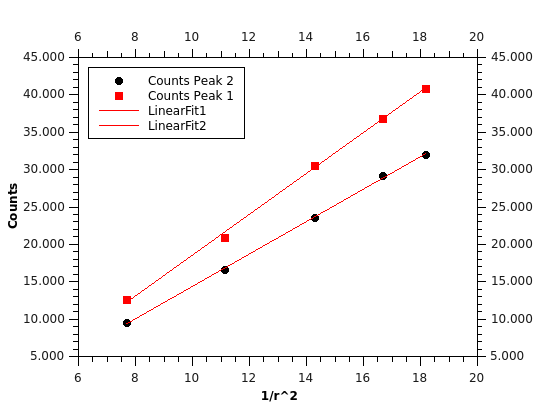
\includegraphics[scale=1.3]{./figures/Endergebniss_Abstand_mitFits.png}
	\caption{Verhältnis von Abstand ($r^2$) zu Ereignisanzahl (ln von Summe über Bereich)}
	\label{fig:abstandsgesetz_erg}
\end{figure}
% TODO lambda? für echte Countes vom intercept e^intercept ;)

% [30.06.14 21:45	Diagramm: ''Grafik1'']
% Lineare Regression von Datensatz: FitIntegralergebnisse_ln(Counts1), unter Verwendung der Funktion: A*x+B
% Gewichtungsmethode: Keine Gewichtung (alle w_i = 1)
% Von x = 5,500000000000000e-02 bis x = 1,300000000000000e-01
% B (y-intercept) = 1,144194727689966e+01 +/- 8,079573075641884e-02
% A (slope) = -1,570157544300322e+01 +/- 9,453188177227960e-01
% --------------------------------------------------------------------------------------
% Chi^2/doF = 3,324294921763869e-03
% R^2 = 0,989242921157287
% Angepasstes R^2 = 0,978485842314573
% RMSE (Standardabweichung) = 0,0576566988455274
% RSS (Summe der quadrierten Restwerte) = 0,00997288476529153
% ---------------------------------------------------------------------------------------
% [30.06.14 21:45	Diagramm: ''Grafik1'']
% Lineare Regression von Datensatz: FitIntegralergebnisse_ln(Counts2), unter Verwendung der Funktion: A*x+B
% Gewichtungsmethode: Keine Gewichtung (alle w_i = 1)
% Von x = 5,500000000000000e-02 bis x = 1,300000000000000e-01
% B (y-intercept) = 1,122650811491831e+01 +/- 6,738920842337341e-02
% A (slope) = -1,613655635448036e+01 +/- 7,884610515636363e-01
% --------------------------------------------------------------------------------------
% Chi^2/doF = 2,312615486978147e-03
% R^2 = 0,992888511500226
% Angepasstes R^2 = 0,985777023000453
% RMSE (Standardabweichung) = 0,048089660915608
% RSS (Summe der quadrierten Restwerte) = 0,00693784646093448
% ---------------------------------------------------------------------------------------
\subsection{Reichweite von Alpha-Strahlen in Luft}

Zerfallsenergie von Ra226: \\
$ZE = (4.870 \pm 0.020)$MeV\\
Reichweite nach der Näherungsformel:
$$R_max =(3.333 \pm 0.021)cm$$
Aus der Messung:
$$R_max = (4.8 \pm 0.5)cm$$

\begin{figure}[H]
	\centering
	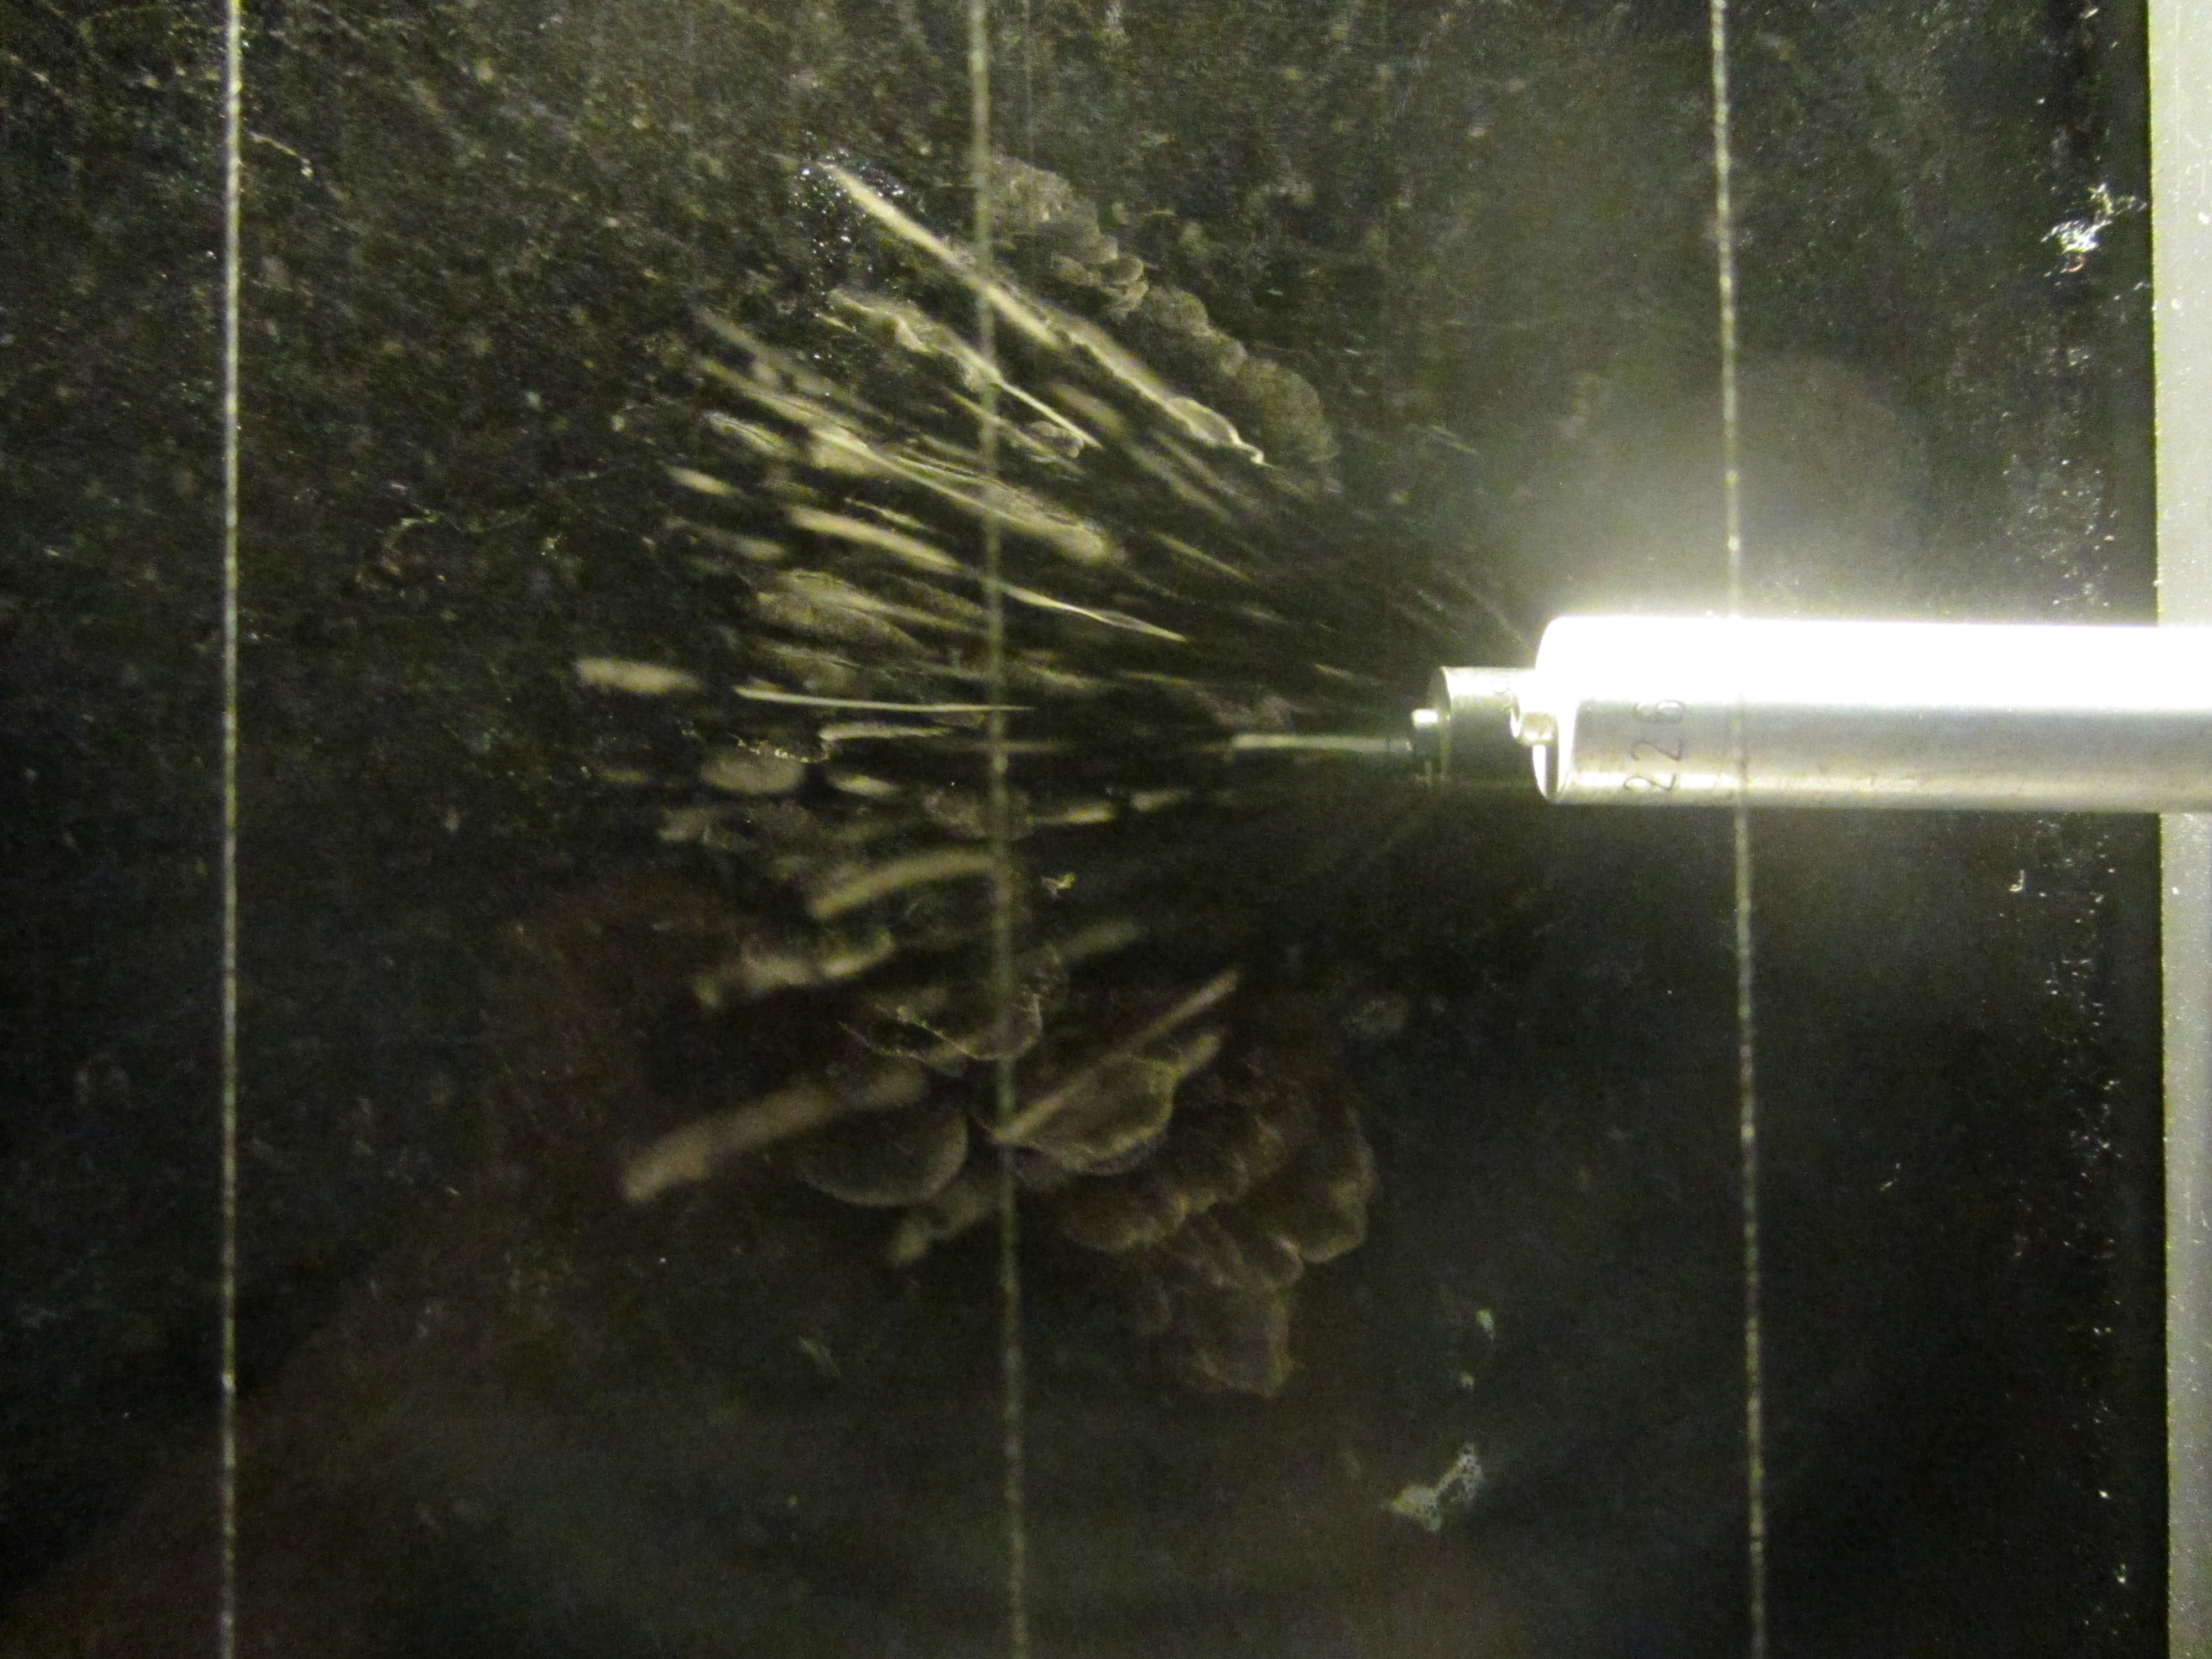
\includegraphics[scale=0.055]{./figures/alpha_auswertung.JPG}
	\caption{Bild der Nebelkammer gefüllt mit Ethanol mit Alphateilchenspur von Radium-226 zerfällen}
	\label{fig:roh_nebel_erg}
\end{figure}

\begin{figure}[H]
	\centering
	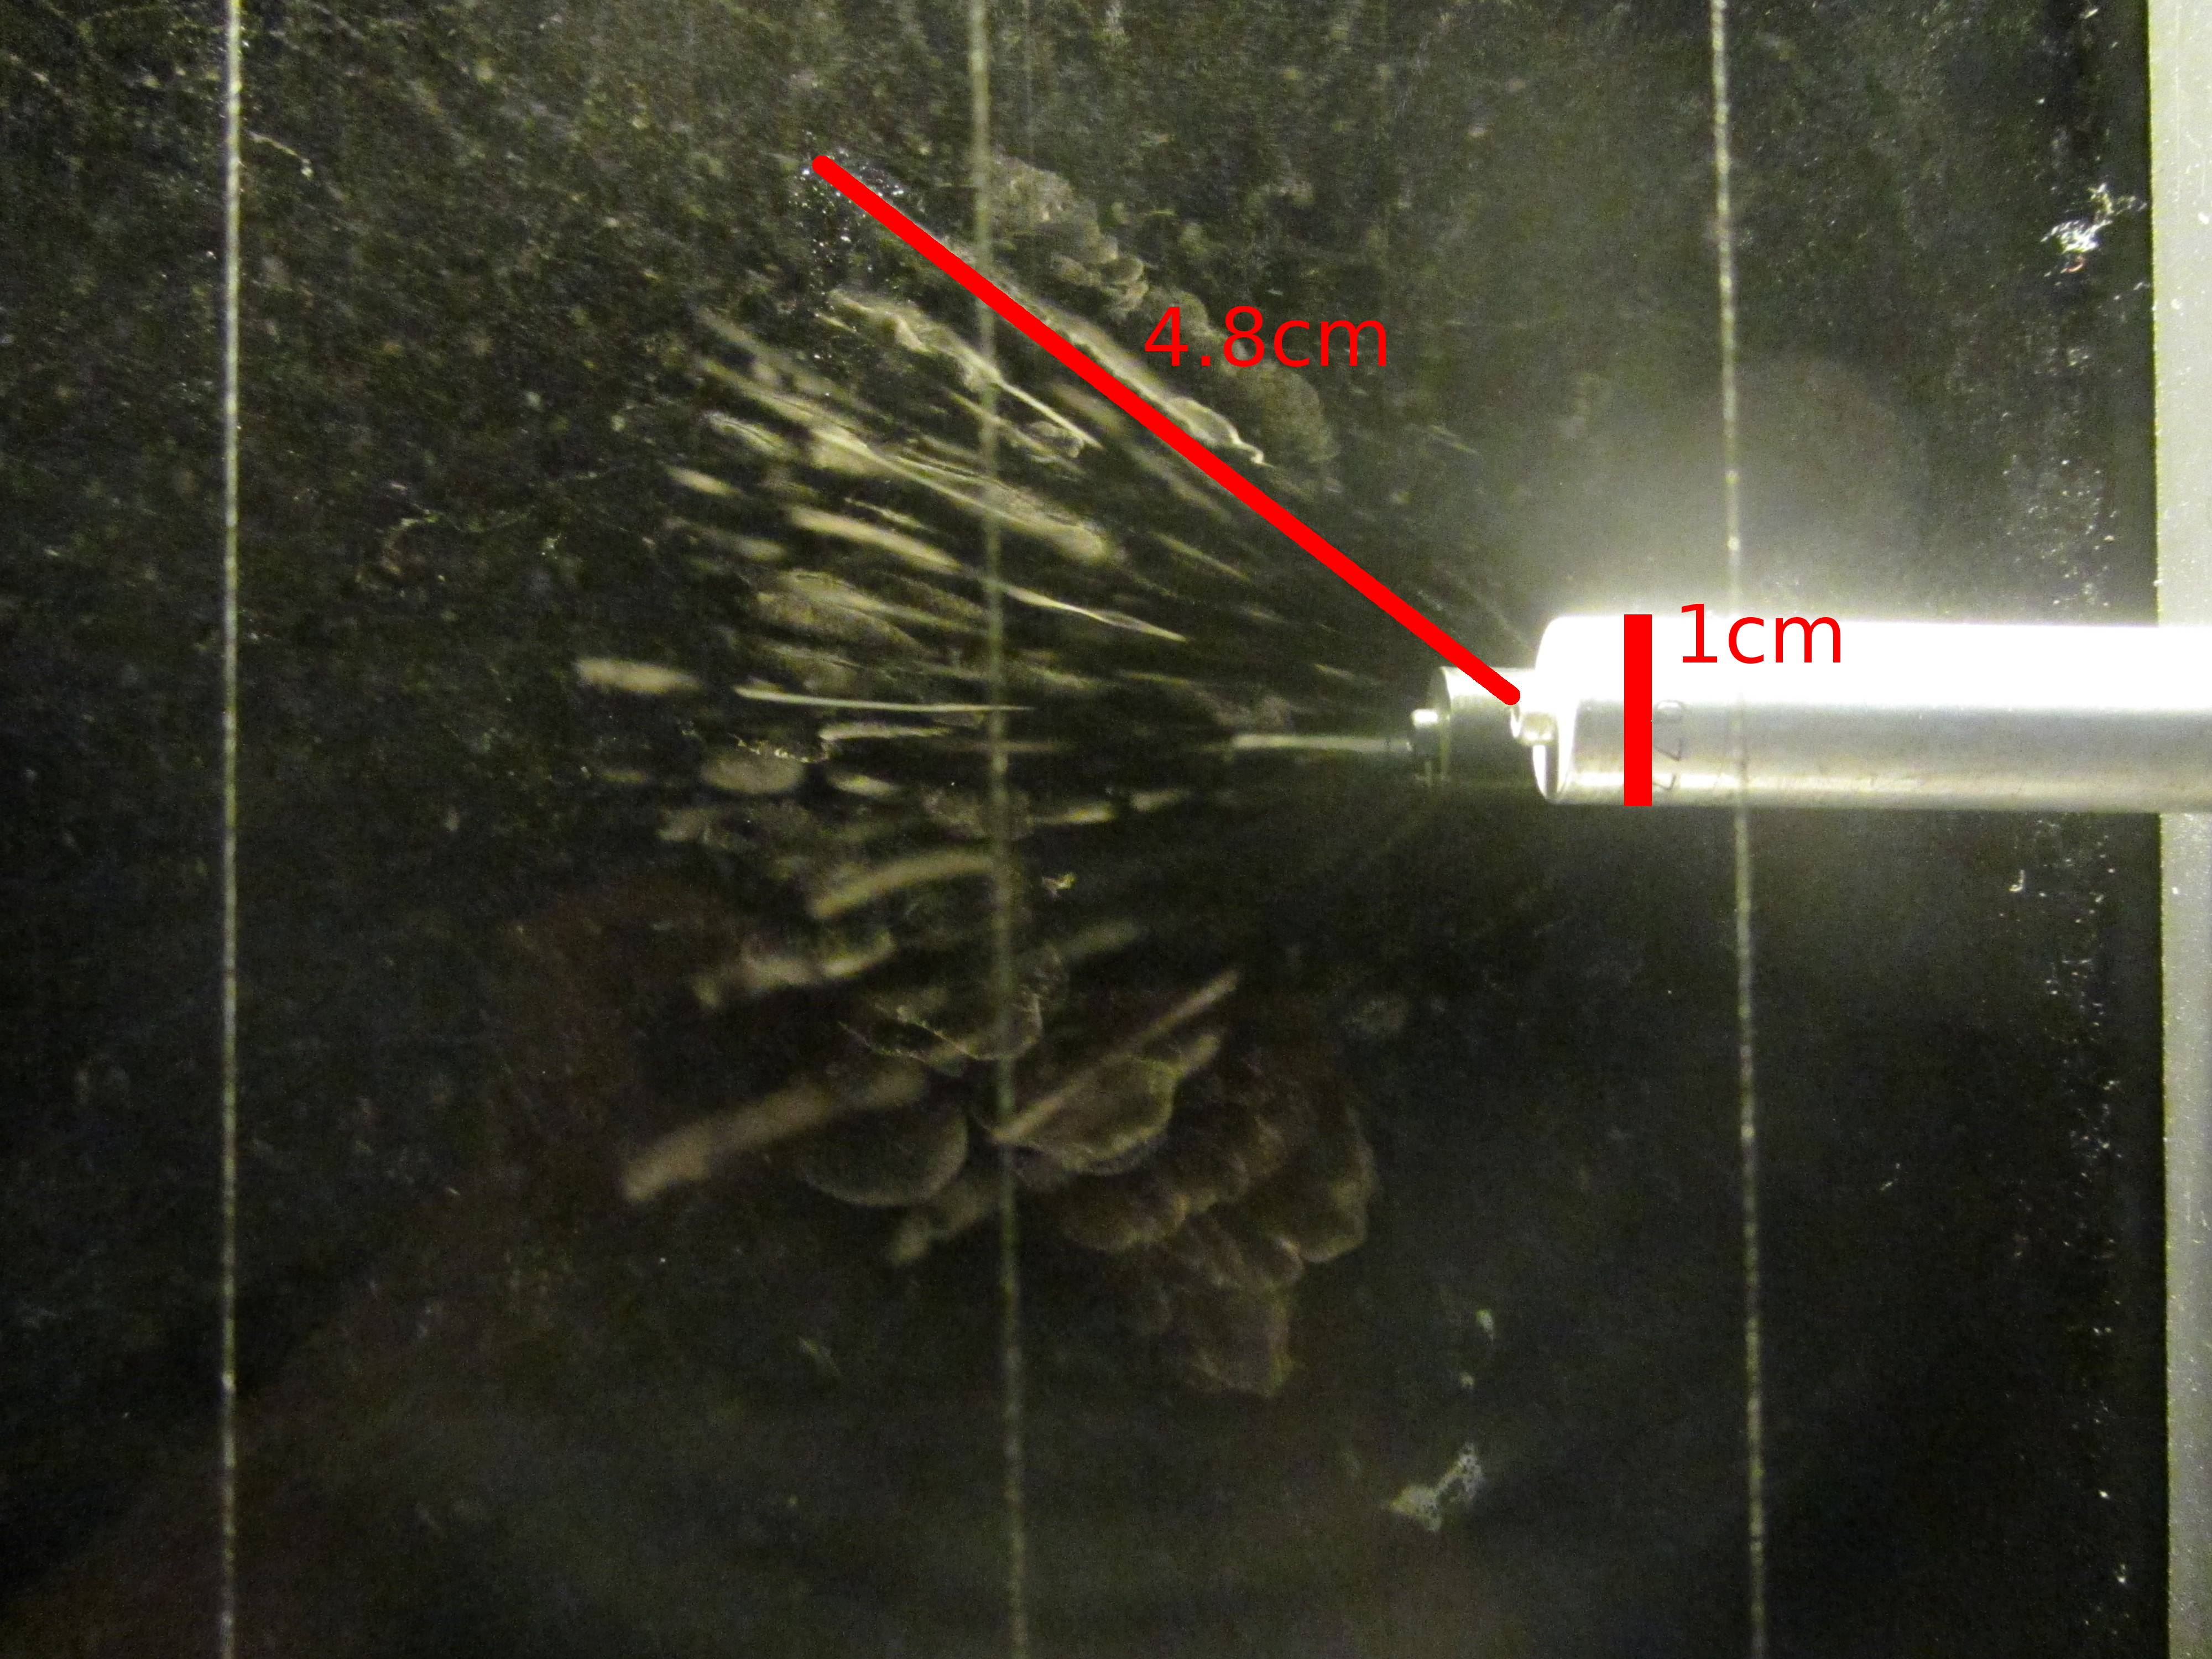
\includegraphics[scale=0.13]{./figures/radium226_ethanol_nebelspur.jpg}
	\caption{Maximale Spurlänge eines Alphateilchens in Ethanol}
	\label{fig:ausw_nebel_erg}
\end{figure}

%%%%%%%%%%%%%%%%%%%%%%%%%%%%%%%%%%%%%%%%%%%%%%%%%%%%%%%%%%%%%%%%%%%%%%%
\pagebreak
\section{Diskussion}

\subsection{Radioaktiver Zerfall von Kupfer}
Die Abschätzung der Körpereigenen Aktivität ist aufgrund der Ausgangsannahmen sehr groß. Da alle verwendeten Werte aus der Angabe stammen oder Literaturwerte sind, wird für das Ergebnis eine Unsicherheit von $10\%$ abgeschätzt. Verglichen mit einer Abschätzung von 5000Bq (Wikipedia; Körpergewicht unbekannt) ist der ermittelte Wert von $(4350 \pm 435) Bq$ plausibel.\\

\noindent Die Messung der Zerfälle der Kupferprobe wurde über die Gesamte Dauer des Praktikums durchgeführt.\\
Daher ist anzunehmen, dass die anderen Versuche (und das Einbringen und entfernen diverser radioaktiver Proben während dieser, sowie die teilweise verwendeten hohen Spannungen) die Zählung verfälschen. Ein einheitlicher systematischer Fehler entsteht dadurch jedoch nicht.\\

\noindent In Abb.\ref{fig:kupferzerfall_erg} ist die große Streuung der gemessenen Zerfälle gut zu erkennen (schon bereinigt durch die anfangs gemessene Hintergrundstrahlung und logarithmiert). Diese entsteht auch durch die statistische Natur des Zerfallsprozesses und der, im Vergleich zur Messdauer von 10 min, nicht riesigen mittleren Lebensdauer von etwa 17.5h.\\

\noindent Im Mittel zeigt sich jedoch, aufgrund der ausreichend langen Messdauer, eine gute Übereinstimmung der gemessenen Halbwertszeit $T_{1/2} = (12.1 \pm 2.1)h$ mit dem
Literaturwert für Cu-64: $T_{1/2} ({64}^{Cu}) = 12.701(2) h$\\

\noindent Gegen Ende des Versuchs wurde gleichzeitig und in der Nähe Aufgabe 4 (Alpha-Teilchen in der Nebelkammer) durchgeführt. Bevor die Kupfermessung mit zusätzlichem Blei abgeschirmt wurde, ergab sich ein deutlicher Ausreisser bei Minute 220, der aus dem Ergebnis entfernt wurde.

\subsection{Beta- und Gammaspektroskopie}

\subsection{Abstandsgesetz für punktförmige Strahler}

\subsection{Reichweite von Alpha-Strahlen in Luft}



%%%%%%%%%%%%%%%%%%%%%%%%%%%%%%%%%%%%%%%%%%%%%%%%%%%%%%%%%%%%%%%%%%%%%%%
\section{Quellen}
$[1]$ Anleitung, \url{http://www.univie.ac.at/anfpra/neu1/ps/ps3/PS3.pdf}\\
$[2]$ Rohdaten, \url{htts://github.com/blackandcold/Protocols-SS2014-P2/tree/master/PS_3/data}\\
$[3]$ Kupfer, \url{http://www.internetchemie.info/chemiewiki/index.php?title=Kupfer-Isotope}
\end{multicols}
\end{document}